\documentclass[11pt]{amsart}
\usepackage[a4paper,textwidth=158mm,textheight=237mm,centering]{geometry}
\usepackage[T1]{fontenc}
\usepackage{lmodern,microtype,mathtools,amssymb,graphicx,flafter,booktabs}
\usepackage[unicode,colorlinks=true,linkcolor=black,citecolor=black,urlcolor=blue]{hyperref}
\newtheorem{theorem}{Theorem}[section]
\newtheorem{lemma}[theorem]{Lemma}
\theoremstyle{remark}
\newtheorem{remark}[theorem]{Remark}
\newcommand{\kk}{\mathbb F_{1009}}
\newcommand{\m}{\mathfrak m}
\newcommand{\Spec}{\operatorname{Spec}}
\newcommand{\Id}{\operatorname{Id}}
\title{The truncated dodecahedron is rigid}
\author{Harvey Yorke}
\address{Valyu AI}
\ifdefined\journalversion\else
\author{Valyu DeepResearch}
\address{Valyu AI}
\fi
\ifdefined\journalversion
  \hypersetup{pdftitle={The truncated dodecahedron is rigid},pdfauthor={Harvey Yorke}}
\else
  \hypersetup{pdftitle={The truncated dodecahedron is rigid},pdfauthor={Harvey Yorke and Valyu DeepResearch}}
\fi
\date{18 October 2026}
\keywords{Polytope rigidity, flat faces, higher-order obstruction, arithmetic specialization}
\newcommand{\paperAuthorBlock}[1]{%
  \begin{minipage}[t]{.44\textwidth}
    \centering\normalfont\normalsize #1\par\small Valyu AI\par
  \end{minipage}%
}
\makeatletter
\renewcommand{\@setauthors}{%
  \begingroup\trivlist\centering\normalfont\normalsize
  \@topsep30\p@\relax\advance\@topsep by -\baselineskip\item\relax
  \ifdefined\journalversion
    \paperAuthorBlock{Harvey Yorke}%
  \else
    \paperAuthorBlock{Harvey Yorke}\hspace{.06\textwidth}\paperAuthorBlock{Valyu DeepResearch}%
  \fi
  \endtrivlist\endgroup
}
\renewcommand{\@setaddresses}{}
\makeatother
\begin{document}
\raggedbottom
\begin{abstract}
The classical truncated dodecahedron is locally rigid when its original edge lengths and the coplanarity of its faces are preserved. These constraints allow the decagonal faces to change shape, so Cauchy's rigidity theorem does not settle the question. A recent second-order analysis leaves this example unresolved. We give an arithmetic certificate: after six Euclidean gauges, the defining equations have four infinitesimal parameters modulo 1009. Their quadratic obstructions vanish, but four cubic obstructions generate an ideal containing the ninth power of each parameter. This proves isolation of the special-fiber point. Openness of the quasi-finite locus along an integral zero section transfers isolation to characteristic zero. The certificate is checked by exact arithmetic without relying on a Gr\"obner-basis engine.
\end{abstract}
\maketitle
\section{The rigidity question}

Adrian-Himmelmann, Winter and Zhang~\cite{AHWZ2026} study deformations of convex polytopes that preserve original edge lengths and face coplanarity. Their second-order method settles the regular dodecahedron and truncated icosahedron, but leaves the truncated dodecahedron unresolved. The latter has four infinitesimal flex parameters after quotienting Euclidean motions, and its second-order obstructions vanish. We resolve this local question by certifying isolation in one finite characteristic and transferring it to the characteristic-zero realization.

\begin{theorem}\label{thm:main}
The classical truncated dodecahedron is locally rigid under deformations preserving its original edge lengths and the coplanarity of every original face. Every sufficiently nearby realization satisfying these constraints is congruent to the original one.
\end{theorem}

The conclusion does not fix face shapes: the decagonal diagonals are unconstrained. It is therefore distinct from Cauchy's theorem for convex polyhedra with congruent corresponding faces. Nor does it assert rigidity of the bare bar graph after the face constraints are removed, or global uniqueness among distant realizations.

The proof has two steps. Exact polynomial identities over $\mathbb F_{1009}$ show that every infinitesimal parameter is nilpotent in the completed local realization ring. The original configuration defines a section over an integral coefficient ring, so openness of the quasi-finite locus carries this isolation to characteristic zero. The second step avoids any assumption that the modular equations or their ranks lift unchanged.

\begin{figure}[ht]
 \centering
 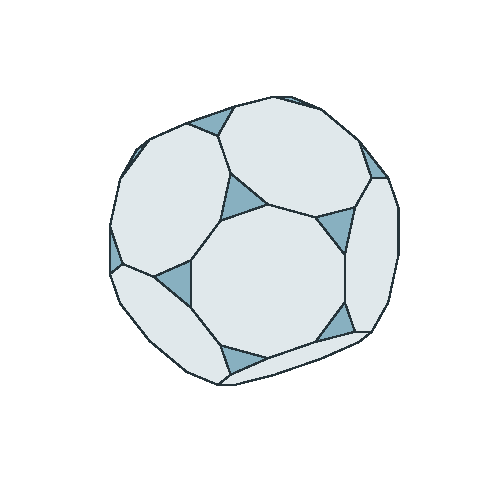
\includegraphics[width=.46\textwidth]{truncated-dodecahedron.pdf}
 \caption{The exact realization used in the certificate, drawn from its saved vertices and facet incidences. It has 60 vertices, 90 original edges, 20 triangular faces and 12 decagonal faces. No face diagonals are added.}
 \label{fig:polytope}
\end{figure}

\section{An integral realization space}

Put $\phi=(1+\sqrt5)/2$. Take cyclic coordinate permutations and independent signs in
\begin{equation}\label{eq:vertices}
 (0,\pm(\phi-1),\pm(\phi+2)),\quad
 (\pm(\phi-1),\pm\phi,\pm2\phi),\quad
 (\pm\phi,\pm2,\pm(\phi+1)).
\end{equation}
Discarding duplicates gives sixty vertices $p_i$. Their original edges have squared length $8-4\phi$. An exact identification with the classical Archimedean solid is useful: start with the twenty standard dodecahedral vertices $(\pm1,\pm1,\pm1)$ and cyclic permutations of $(0,\pm(\phi-1),\pm\phi)$. For every directed dodecahedral edge $a\to b$, form $\phi a+(\phi-1)b$. The resulting set is precisely~\eqref{eq:vertices}. Dividing by $\sqrt5$ gives uniform truncation fraction $1/(\phi+2)$, for which the shortened old edges and new cut edges have equal length.

For each facet $f$, normalize its outward normal $a_f$ by $p_i\cdot a_f=1$ on that facet. The saved coefficients lie in $\mathbb Z[\phi,1/55]$. Exact supporting-plane inequalities verify the thirty-two faces; a separate check verifies regular triangles and regular decagons. Thus the numerical convex hull used to propose incidences is not trusted as part of the certificate.

There are 276 variables: the three coordinates of each of the sixty vertices and thirty-two normalized normals. Translate the original configuration to $u=0$. The ninety edge equations and 180 incidence equations are
\begin{align}
 \|p_i+u_i-p_j-u_j\|^2-\|p_i-p_j\|^2&=0 &&(ij\in E),\label{eq:edges}\\
 (p_i+u_i)\cdot(a_f+u_f)-1&=0 &&(i\in f).\label{eq:incidence}
\end{align}
Over $\mathbb C$, the squared norm denotes the same polynomial quadratic form, without complex conjugation.

Fix displacement coordinates $0,1,2,3,4,6$ in the saved vertex ordering. These six linear gauges are transverse to Euclidean motions: the corresponding six-by-six derivative has determinant of absolute value $4$ over $\mathbb Q(\phi)$. With the gauges included, write the 276 equations as
\[
 F(u)=J_0u+q(u),
\]
where $q$ is homogeneous quadratic. All coefficients belong to the integral domain
\begin{equation}\label{eq:base}
 A=\mathbb Z[\phi,1/55],\qquad \phi^2-\phi-1=0.
\end{equation}
The equations define a finite-type scheme $X\to\Spec A$. Since $F(0)=0$ identically, $u=0$ defines a section $\sigma:\Spec A\to X$.

\section{The finite-field certificate}

Reduce~\eqref{eq:base} at the prime $(1009,\phi-627)$. Both $627^2-627-1=0$ and $55\ne0$ hold in $\kk$. The following data are verified by the supplied independent checker. All linear algebra in this section is over $\kk$.

\begin{center}
\begin{tabular}{ll}
\toprule
Certificate quantity & Verified value\\
\midrule
Variables and equations after gauges & $276$, $276$\\
Jacobian rank & $272$\\
Kernel and left-nullspace dimensions & $4$, $4$\\
Quadratic obstruction coefficients & $40$ zeros\\
Cubic obstruction coefficients reconstructed & $80$\\
Pure-power identities & $v_i^9=\sum_{j=1}^4 A_{ji}C_j$\\
Multiplier degrees & $\deg A_{ji}=6$\\
\bottomrule
\end{tabular}
\end{center}

Let $J$ be the reduced Jacobian. The certificate supplies a kernel matrix $K$ with four columns, a pivot-coordinate inclusion $I$ with 272 columns, a 272-row matrix $R$, and a four-row left-null matrix $L$. They satisfy
\begin{equation}\label{eq:linear}
 JK=0,\qquad RJI=\Id_{272},\qquad LJ=0.
\end{equation}
The four free rows of $K$ form the identity and the rows of $L$ are independent. Hence $(v,w)\mapsto Kv+Iw$ and the stacked equation transformation $(R;L)$ are invertible. In the coordinates $(v,w)$, the range equations $RF(Kv+Iw)=0$ have linear part $w$.

\begin{lemma}\label{lem:formal}
The completed local ring of the special fiber at $\sigma(p)$ is
\[
 B=\kk[[v_0,v_1,v_2,v_3]]/(g_1,g_2,g_3,g_4),
\]
where $g_j=C_j+O((v)^4)$ and the $C_j$ are the certified homogeneous cubics.
\end{lemma}
\begin{proof}
The formal change $(v,w)\mapsto(v,RF(Kv+Iw))$ has identity linear part and is an automorphism of the power-series ring. Equivalently, the formal implicit-function theorem gives a unique $w(v)=w_2(v)+O((v)^3)$. This works over any field; see~\cite[Tag 07NM]{Stacks}. Completion commutes with the finite quotient defining the local ring~\cite[Tag 00MA]{Stacks}.

The saved homogeneous quadratic vector $W_2$, supported in the pivot coordinates, satisfies
\begin{equation}\label{eq:correction}
 JW_2(v)+q(Kv)=0.
\end{equation}
It is therefore $Iw_2(v)$. In particular, $Lq(Kv)=0$. After eliminating $w$, the four complementary series are $g(v)=LF(Kv+Iw(v))$. Since $LJ=0$, their cubic part is exactly
\begin{equation}\label{eq:cubics}
 C(v)=L\bigl[q(Kv+W_2(v))-q(Kv)-q(W_2(v))\bigr].
\end{equation}
The checker reconstructs every coefficient of~\eqref{eq:cubics} from the original equations. All omitted terms have degree at least four.
\end{proof}

\begin{lemma}\label{lem:isolated}
The special-fiber point $\sigma(p)$ is isolated.
\end{lemma}
\begin{proof}
Write $S=\kk[[v_0,v_1,v_2,v_3]]$, $\m=(v_0,v_1,v_2,v_3)$ and $J_g=(g_1,g_2,g_3,g_4)$. Direct polynomial multiplication verifies the four identities
\begin{equation}\label{eq:powers}
 v_i^9=\sum_{j=1}^4 A_{ji}(v)C_j(v),\qquad 0\le i\le3,
\end{equation}
with each $A_{ji}$ homogeneous of degree six. Since $g_j-C_j\in\m^4$, these imply $v_i^9\in J_g+\m^{10}$. Every monomial of degree 33 is divisible by some $v_i^9$: four exponents at most eight have sum at most 32. Thus
\[
 \m^{33}\subset J_g+\m^{34}.
\]
In the Noetherian local ring $B=S/J_g$, the maximal ideal $\mathfrak n$ consequently satisfies $\mathfrak n^{33}=\mathfrak n\mathfrak n^{33}$. Nakayama's lemma gives $\mathfrak n^{33}=0$, so $B$ is Artinian. Completion preserves local dimension~\cite[Tags 00DV and 07NV]{Stacks}. Therefore the original special-fiber local ring has dimension zero, and its rational closed point is isolated~\cite[Tag 01TH]{Stacks}.
\end{proof}

Only the finite identities~\eqref{eq:powers}, not a claim about the correctness of a Gr\"obner-basis computation, are needed. In particular, arbitrary terms of degree at least four in the reduced equations cannot restore a local branch.

\section{Transfer to characteristic zero and rigidity}

\begin{lemma}\label{lem:transfer}
The zero-section point of the gauge-fixed complex realization space is isolated.
\end{lemma}
\begin{proof}
Let $U\subset X$ be the locus where $X\to\Spec A$ is quasi-finite. This locus is open~\cite[Tag 01TI]{Stacks}. By Lemma~\ref{lem:isolated} and the equivalence between isolated fiber points and quasi-finiteness at a point~\cite[Tag 01TH]{Stacks}, it contains $\sigma(p)$. Thus $\sigma^{-1}(U)$ is a nonempty open subset of the integral scheme $\Spec A$. It contains the generic point $\eta$, and $\sigma(\eta)$ is isolated in the $\mathbb Q(\phi)$ fiber. Quasi-finiteness at points is stable under base change~\cite[Tag 01TM]{Stacks}. Extending through the positive real embedding $\mathbb Q(\phi)\hookrightarrow\mathbb C$ proves the claim.
\end{proof}

The section is essential: it tracks the actual configuration across characteristics. This proof does not lift the modular cubic identities coefficientwise. It requires neither flatness nor properness, and does not assume that Jacobian rank or quadratic obstructions agree in characteristics zero and 1009.

\begin{proof}[Proof of Theorem~\ref{thm:main}]
The six gauges have invertible derivative on the space of Euclidean motions. The real implicit-function theorem places every sufficiently nearby vertex configuration uniquely into the gauge slice by a nearby Euclidean motion. Normalization of facet normals is compatible with this operation: for $p\mapsto Rp+t$,
\[
 a\mapsto\frac{Ra}{1+(Ra)\cdot t}.
\]
The denominator is nonzero near the identity. Each original face contains three affinely independent vertices and avoids the origin, so its normalized normal is uniquely and continuously determined for nearby coplanar realizations. Every allowed nearby polytope consequently gives a nearby solution of~\eqref{eq:edges}--\eqref{eq:incidence}, and hence a solution in the gauge slice. Lemma~\ref{lem:transfer} makes that solution the original one. This proves local rigidity modulo Euclidean motions.

It also excludes a nontrivial continuous deformation starting at the solid. Along such a path, the set of times at which the configuration is congruent to the original is open by local rigidity and closed by continuity of all pairwise distances. Since it contains the initial time, it is the entire interval.
\end{proof}

\newpage
\section{Reproduction and scope of verification}

The certificate includes exact vertex and normal coordinates, original edges and facet incidences, the matrices in~\eqref{eq:linear}, the correction~\eqref{eq:correction}, the cubics~\eqref{eq:cubics}, and the coefficients in~\eqref{eq:powers}. The independent Python checker uses only its standard library and imports no generator code. It reconstructs the original geometry and polynomial coefficients, verifies all 1740 strict off-face supporting inequalities, checks regular faces and the dodecahedral truncation identification, and verifies the linear, quadratic, cubic and pure-power identities. Its successful run and input hashes are retained alongside the certificate. The generator's floating-point hull and optional Singular calculation are unnecessary for this replay.

The checker establishes finite algebraic identities. Lemmas~\ref{lem:formal}--\ref{lem:transfer} and the Euclidean-slice argument supply their mathematical interpretation; these deductions have independent written review but are not formalized in a proof assistant. The independent reconstruction passes for the saved certificate. A broader literature audit and external review are separate from arithmetic verification.

The source~\cite{AHWZ2026} supplies the model and the second-order obstruction result; the specialization and local-algebra machinery are standard. The contribution is the certified resolution of this specific realization. It does not introduce a general new rigidity criterion.

\paragraph{Research assistance.}
Valyu DeepResearch identified the source's open example, suggested higher-order reduction and supplied a numerical lead. Coding agents subsequently developed the exact certificate, the specialization argument and independent verification code, and drafted and revised this manuscript. Further agent reviews checked the deductions and the scope of the source question. These reviews are internal checks and do not constitute external peer review.

\smallskip
\noindent\textbf{Reproduction.} Run the following from this directory:
\begin{quote}\small\ttfamily
python3 -B -O verification/independent\_verification.py
\end{quote}
Run \texttt{sh build.sh} to rebuild both author variants using the supplied diagram. The optional flag \texttt{--redraw-figure} regenerates that illustration. Certificate data, replay records and their input hashes are in \path{verification/}.

\bibliographystyle{plain}
\bibliography{references}
\end{document}
